\setcounter{equation}{0}
\chapter{Results}
\label{chap:results}

\section{Parameters' Initial Values}

In order to define the ranges of \tauh, \vrot and \vout, it is necessary to refer to observational constraints. The common values for typical LAEs are in Tab. \ref{tab:values}. I run CLARA for all the permutations of these 3 parameters. \\

\begin{table}[htbp]
	\centering
	\begin{tabular}{|c|c|c|}
		\hline
		\bv{\tau_{\mathrm{H}}} & \bv{v_{rot}} (\kms) & \bv{v_{out}} (\kms) \\
		\hline
		$10^5$, $10^6$, $10^7$ & 50, 100 & 5, 10, 15, 20, 25, 50, 75 \\
		\hline
	\end{tabular}
	\caption{\textbf{Parameters' Values:} All consistent with a LAE's typical properties}
	\label{tab:values}
\end{table}

The resulting sets of spectra are in Figs. \ref{fig:3_tau10E5_phi83-90}, \ref{fig:3_tau10E7_phi83-90} and \ref{fig:3_tau10E6_phi83-90} for $\theta \simeq 90^\circ$. I do not include the spectra for \vout = 50, 75 \kms because they are the same as \vout = 25 \kms. For this reason, I limit in all the plots \vout to a maximum value of 25 \kms. Nevertheless, the figures for \vout = 50, 75 \kms are in the Appendix \ref{first_plots} in Figs. \ref{fig:2_tau10E5_phi83-90}, \ref{fig:2_tau10E6_phi83-90} and \ref{fig:2_tau10E7_phi83-90}.\\

\newpage

\begin{figure}[h!]
	\begin{center}
		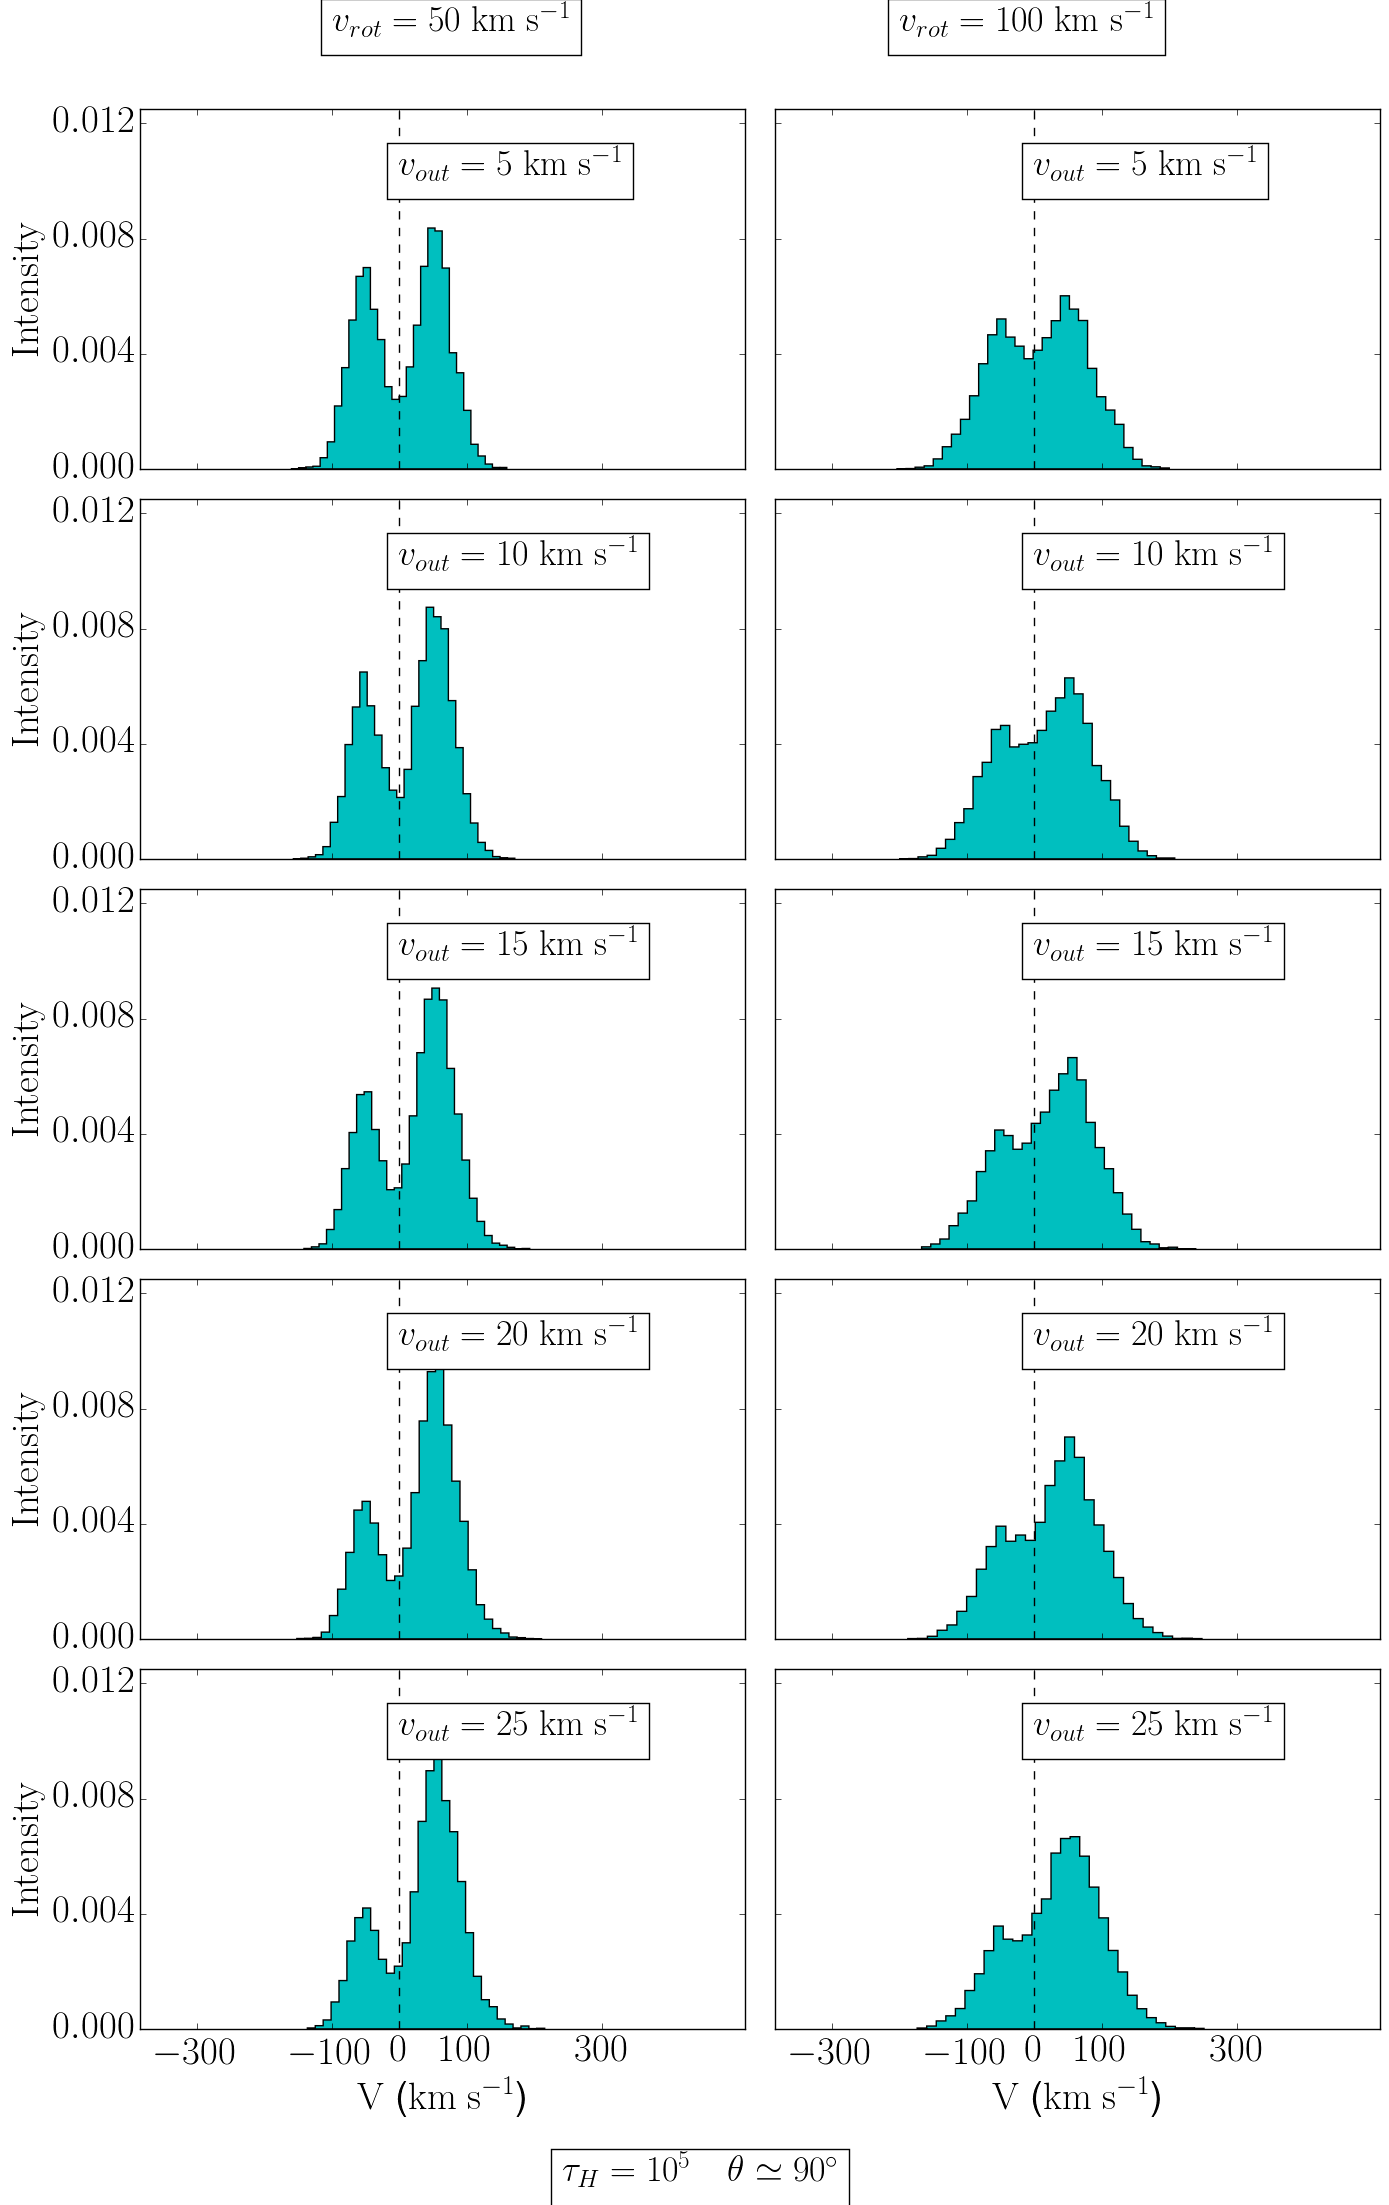
\includegraphics[height=0.8\textheight]{./figures/chapter3/3_tau10E5_phi83-90}
	\end{center}
	\caption{\textbf{\lya profile for \tauh$=10^5$:} With \vrot ranging $50,100$ \kms and \vout ranging $5,10,15,20,25$ \kms. The intensity is in arbitrary units. The viewing angle $\theta \simeq 90^\circ$. The dashed vertical line indicates the \lya line's natural frequency. 
		\label{fig:3_tau10E5_phi83-90}}
\end{figure}

\newpage

\begin{figure}[h!]
	\begin{center}
		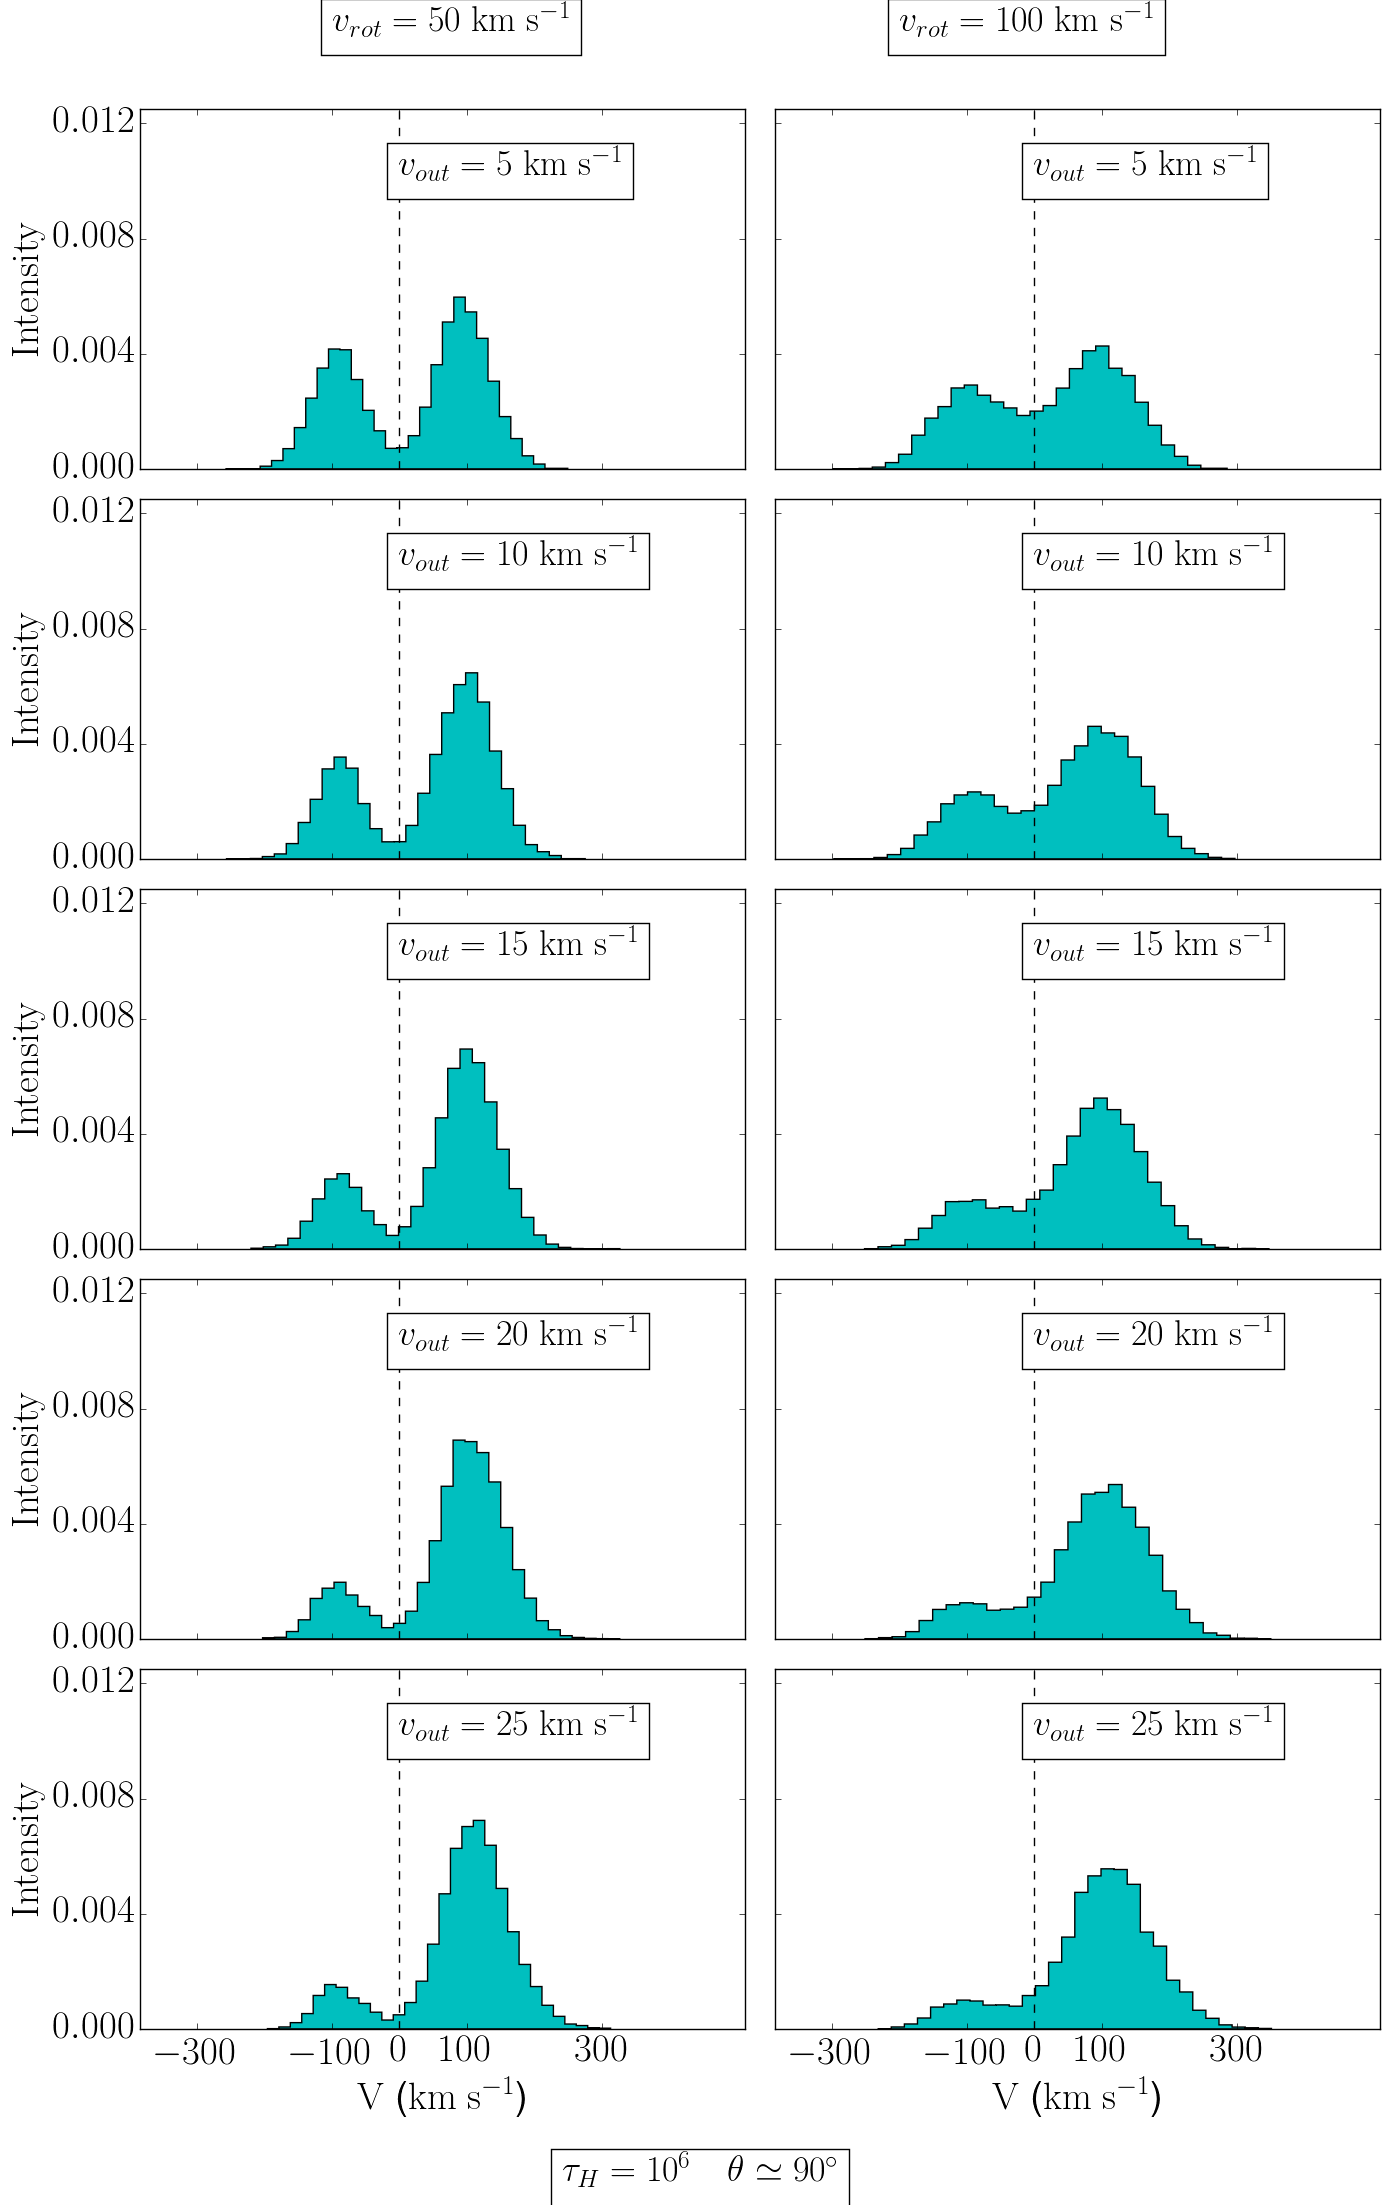
\includegraphics[height=0.8\textheight]{./figures/chapter3/3_tau10E6_phi83-90}
	\end{center}
	\caption{\textbf{\lya profile for \tauh$=10^6$:}  Same as Fig. \ref{fig:3_tau10E5_phi83-90} but for \tauh$=10^6$.
		\label{fig:3_tau10E6_phi83-90}}
\end{figure}

\newpage

\begin{figure}[h!]
	\begin{center}
		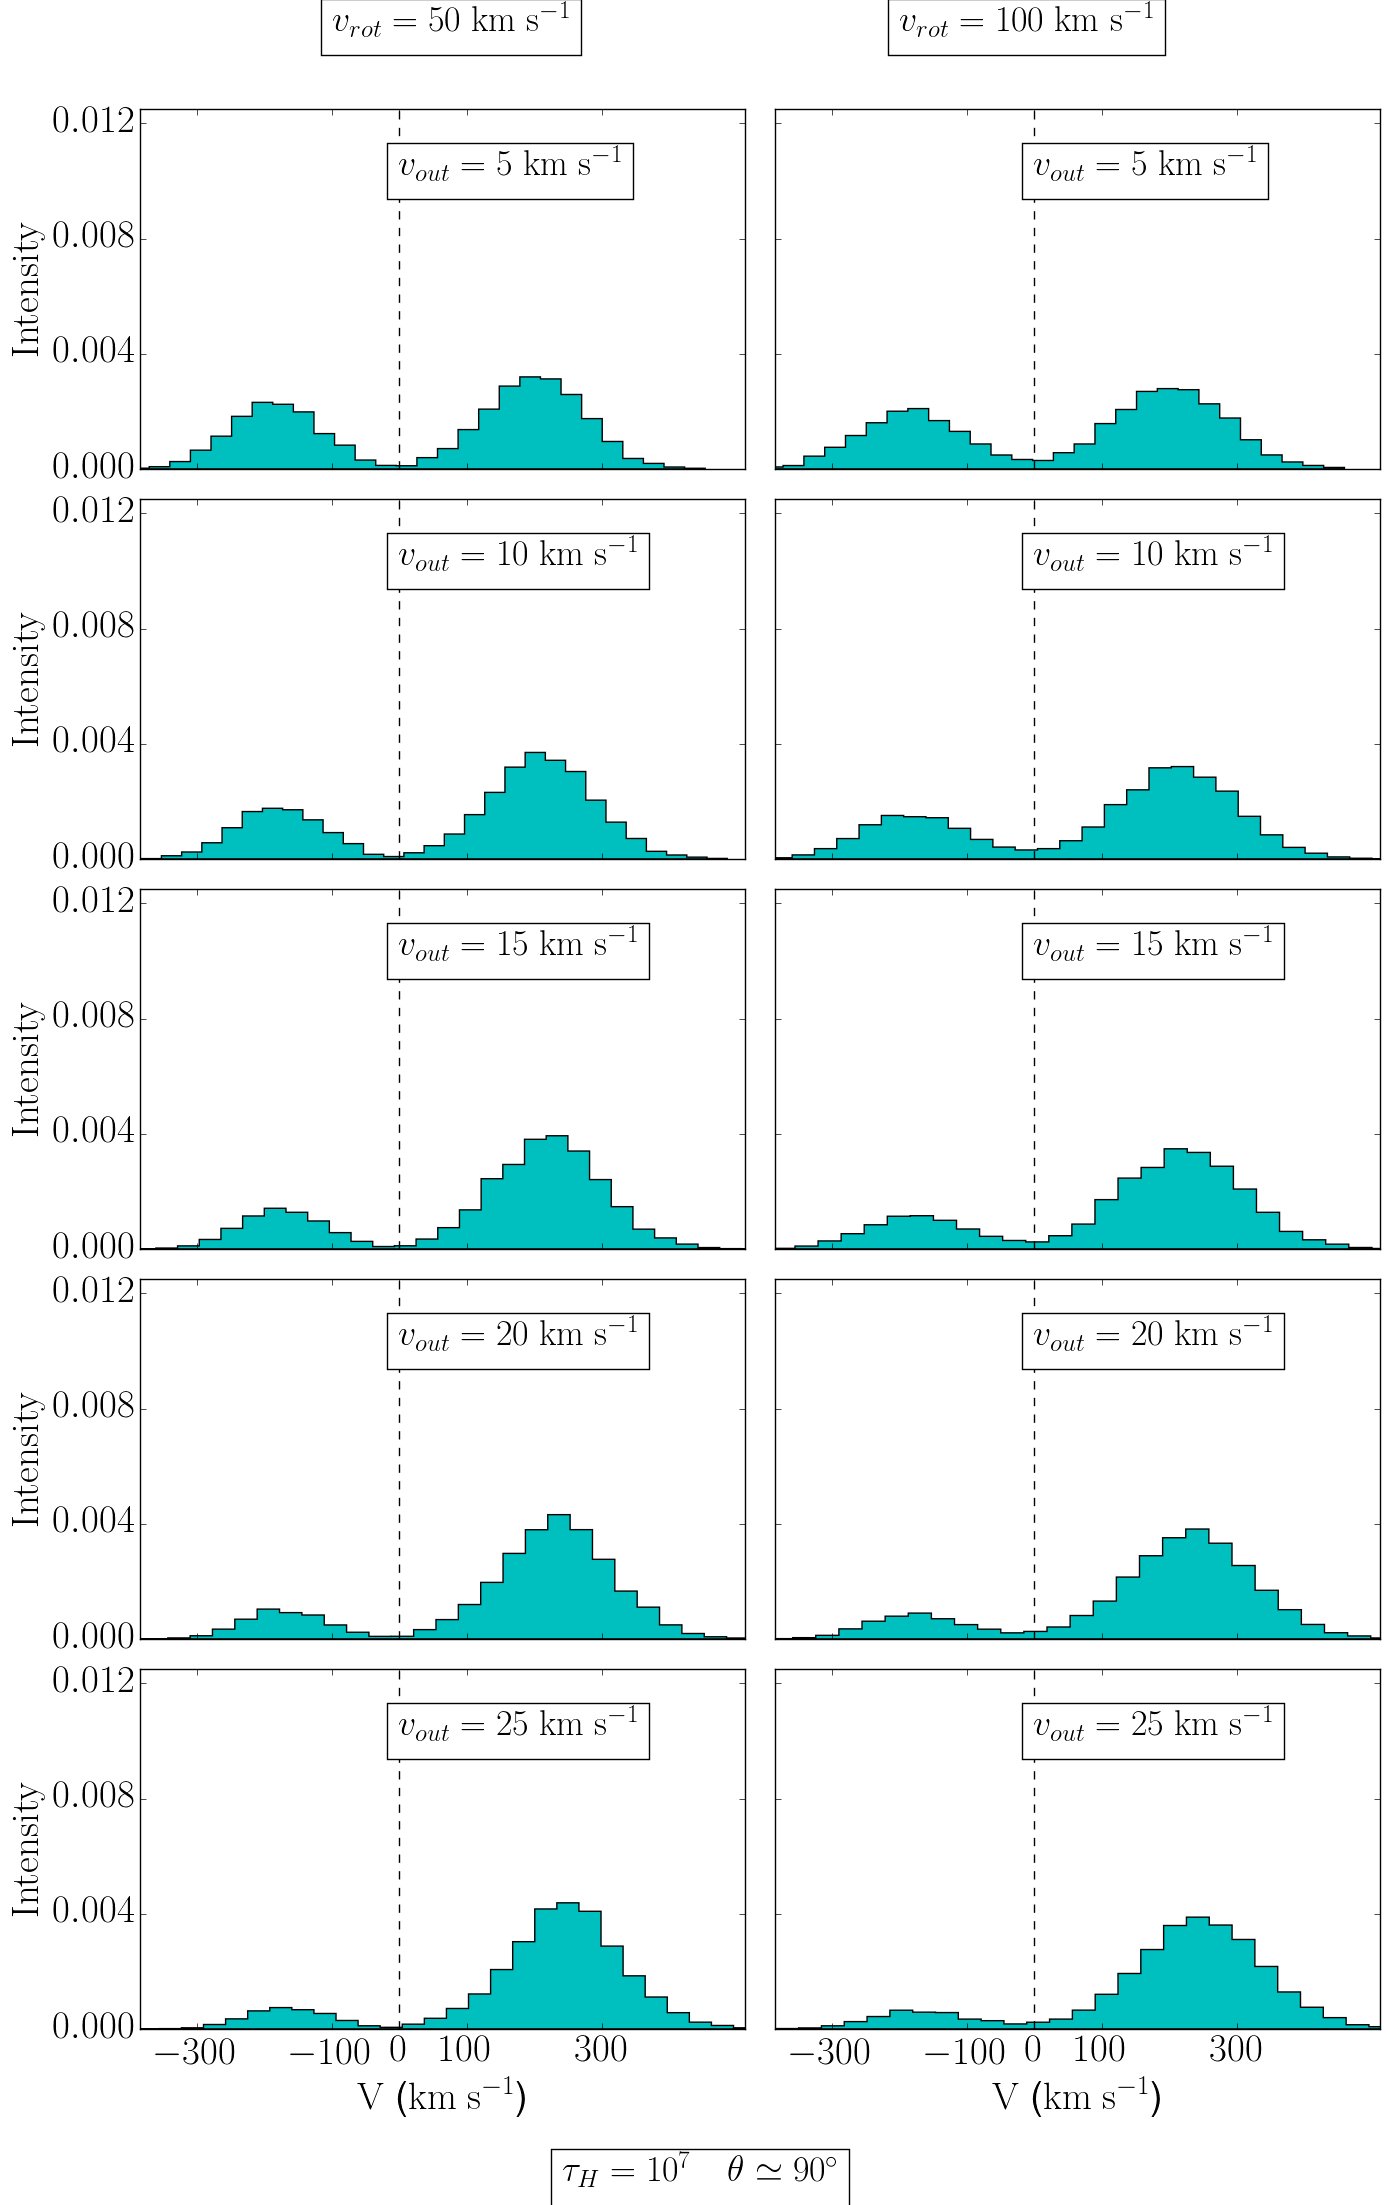
\includegraphics[height=0.8\textheight]{./figures/chapter3/3_tau10E7_phi83-90}
	\end{center}
	\caption{\textbf{\lya profile for \tauh$=10^7$:} Same as Fig. \ref{fig:3_tau10E5_phi83-90} but for \tauh$=10^7$.
		\label{fig:3_tau10E7_phi83-90}}
\end{figure}

\newpage

These last 3 plots show a clear creation of two asymmetric peaks around $V=0$ \kms with the tallest peak is always redshifted, with a strong dependence on the outflow velocity.\\

\section{Influence of the viewing angle $\theta$}
I take now into account the viewing angle of the galaxy to build the observed spectra. For all of the physical parameters' combinations, the effect of $\theta$ in the \lya line is always the same.\\

\begin{figure}[h!]
	\begin{center}
		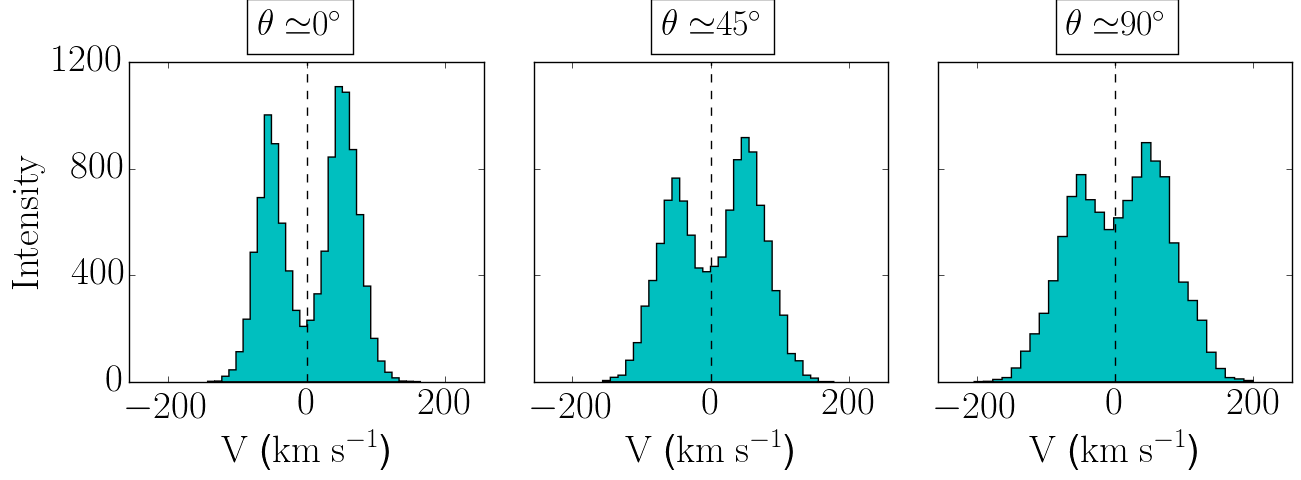
\includegraphics[width=1\textwidth]{./figures/chapter3/influence_viewing_angle_5}
	\end{center}
	\caption{\textbf{\lya profile for different $\theta$:} With \tauh$=10^5$, \vrot$=50$ \kms and \vout$=20$ \kms.The intensity is in arbitrary units.
		\label{fig:influence_viewing_angle_5}}
\end{figure}

\begin{figure}[h!]
	\begin{center}
		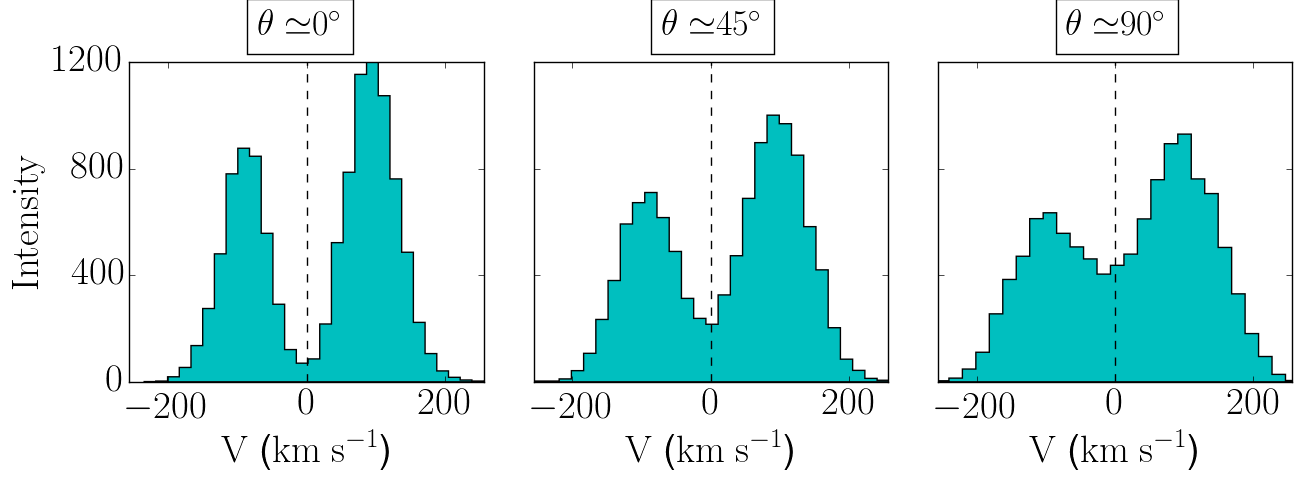
\includegraphics[width=1\textwidth]{./figures/chapter3/influence_viewing_angle_6}
	\end{center}
	\caption{\textbf{\lya profile for different $\theta$:} With \tauh$=10^6$, \vrot$=100$ \kms and \vout$=5$ \kms.The intensity is in arbitrary units.
		\label{fig:influence_viewing_angle_6}}
\end{figure}

\begin{figure}[h!]
	\begin{center}
		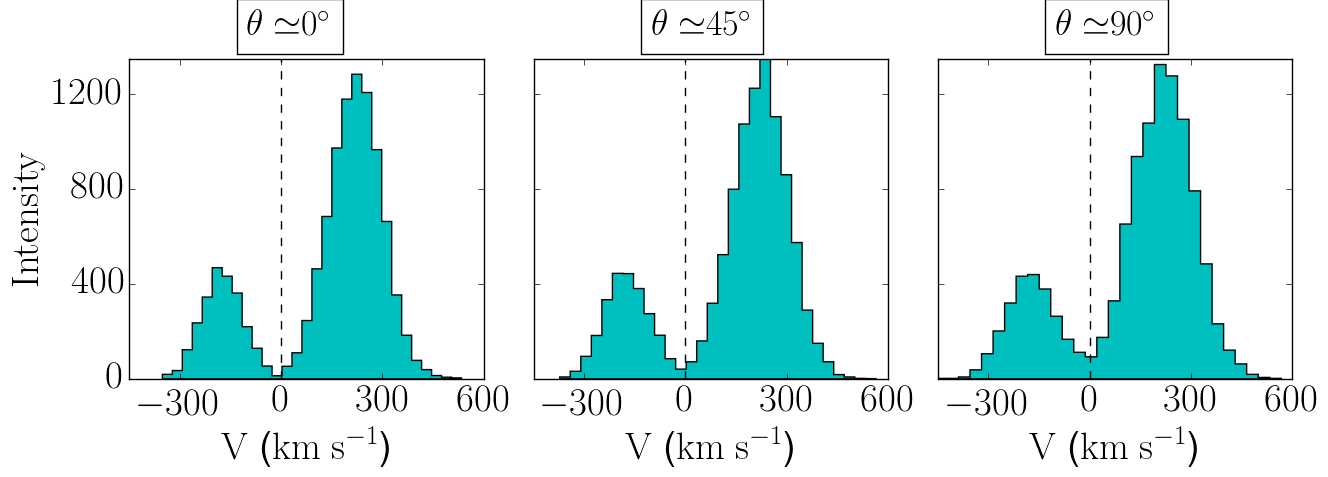
\includegraphics[width=1\textwidth]{./figures/chapter3/influence_viewing_angle_7}
	\end{center}
	\caption{\textbf{\lya profile for different $\theta$:} With \tauh$=10^7$, \vrot$=100$ \kms and \vout$=15$ \kms.The intensity is in arbitrary units.
		\label{fig:influence_viewing_angle_7}}
\end{figure}

From Figs. \ref{fig:influence_viewing_angle_5}, \ref{fig:influence_viewing_angle_6} and \ref{fig:influence_viewing_angle_7} is clear that the intensity of the valley between the two peaks increases along with $\theta$. This causes an intensity decrease in the rest of the frequencies, thus a broadening of the line. The asymmetry also changes with the viewing angle.\\

In the next subsection, I show only the results of the angle at which an observer sees the galaxy's angular momentum vector perpendicular to the line of sight. The purpose of this is only to decrease the number of plots in the document, as there is an analogous behavior for all viewing angles. \\

\section{Morphology of \lya line}
To quantify the morphology of the \lya profile, I use three statistics: the standard deviation, the skewness and a factor sigma of asymmetry ($\sigma_A$). \\

\subsection{Standard Deviation}
The standard deviation measures the dispersion of frequencies in the \lya line. If it increases, the frequencies spread to wider ranges. \\

\begin{figure}[h!]
	\begin{center}
		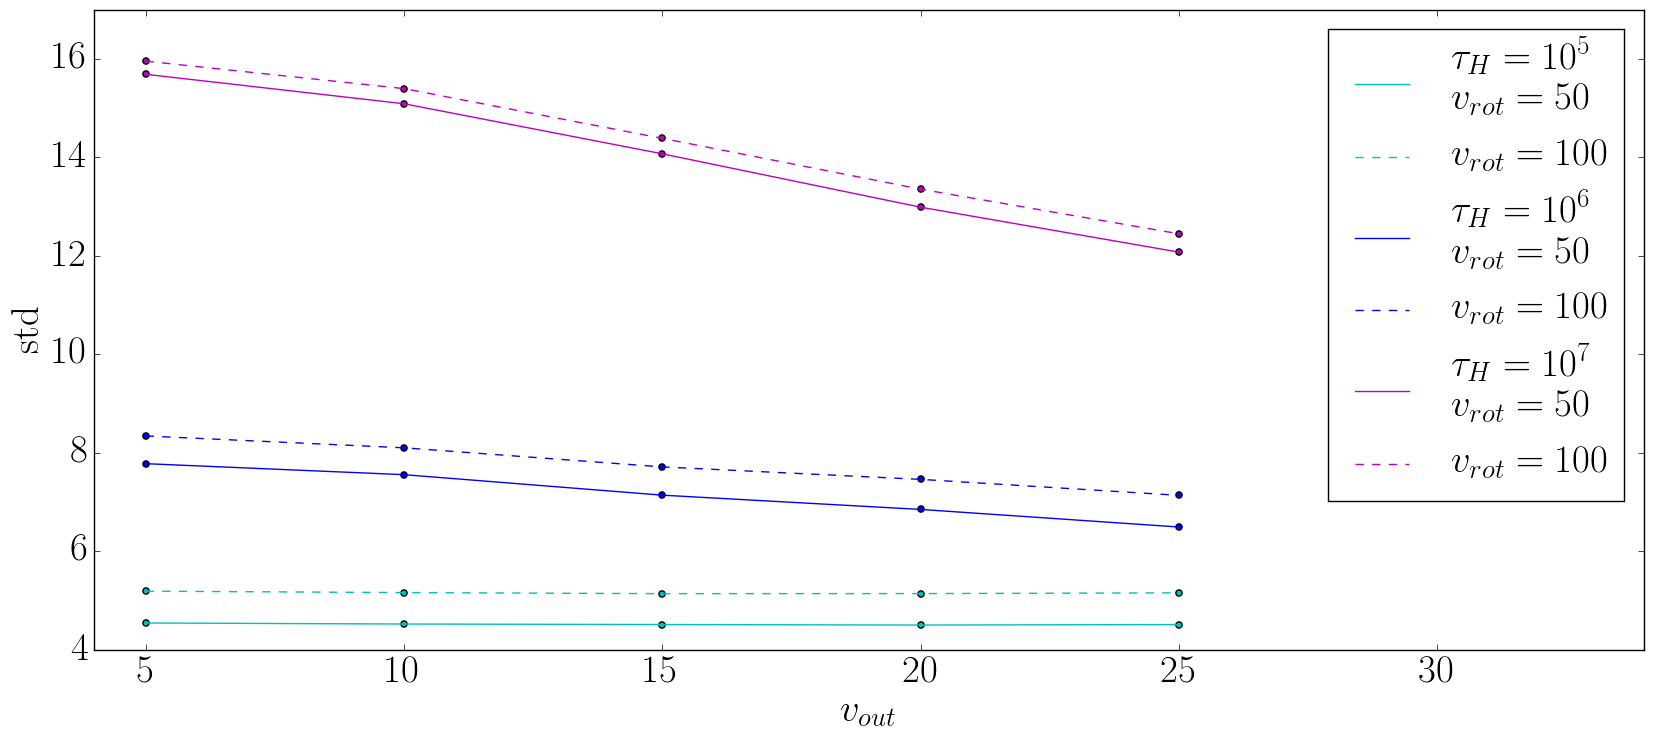
\includegraphics[width=1\textwidth]{./figures/chapter3/std}
	\end{center}
	\caption{\textbf{Standard deviation plot for each \tauh.} The viewing angle $\theta \simeq 90^\circ$.
	\label{fig:std}}
\end{figure}

Fig. \ref{fig:std} shows that the standard deviation is inversely proportional to the outflow velocity. This implies that the greater \vout is, the less disperse is the \lya frequency distribution. This signals that the peaks start merging to one another. Also, the higher the \tauh, the more inclined the curves. The horizontal dotted line in the plot is the value of standard deviation for an observational LAE, in particular Q2206BX151 (at redshift $z\approx2.1974$). It is shown in Fig. \ref{fig:kulas} in the third column with second row. \\

\subsection{Skewness}
The skewness measures the asymmetry of the \lya line. If the value is greater than zero, there is more weight in the left tail of the line, if it is less than zero, there is more weight in the right one.\\

\begin{figure}[h!]
	\begin{center}
		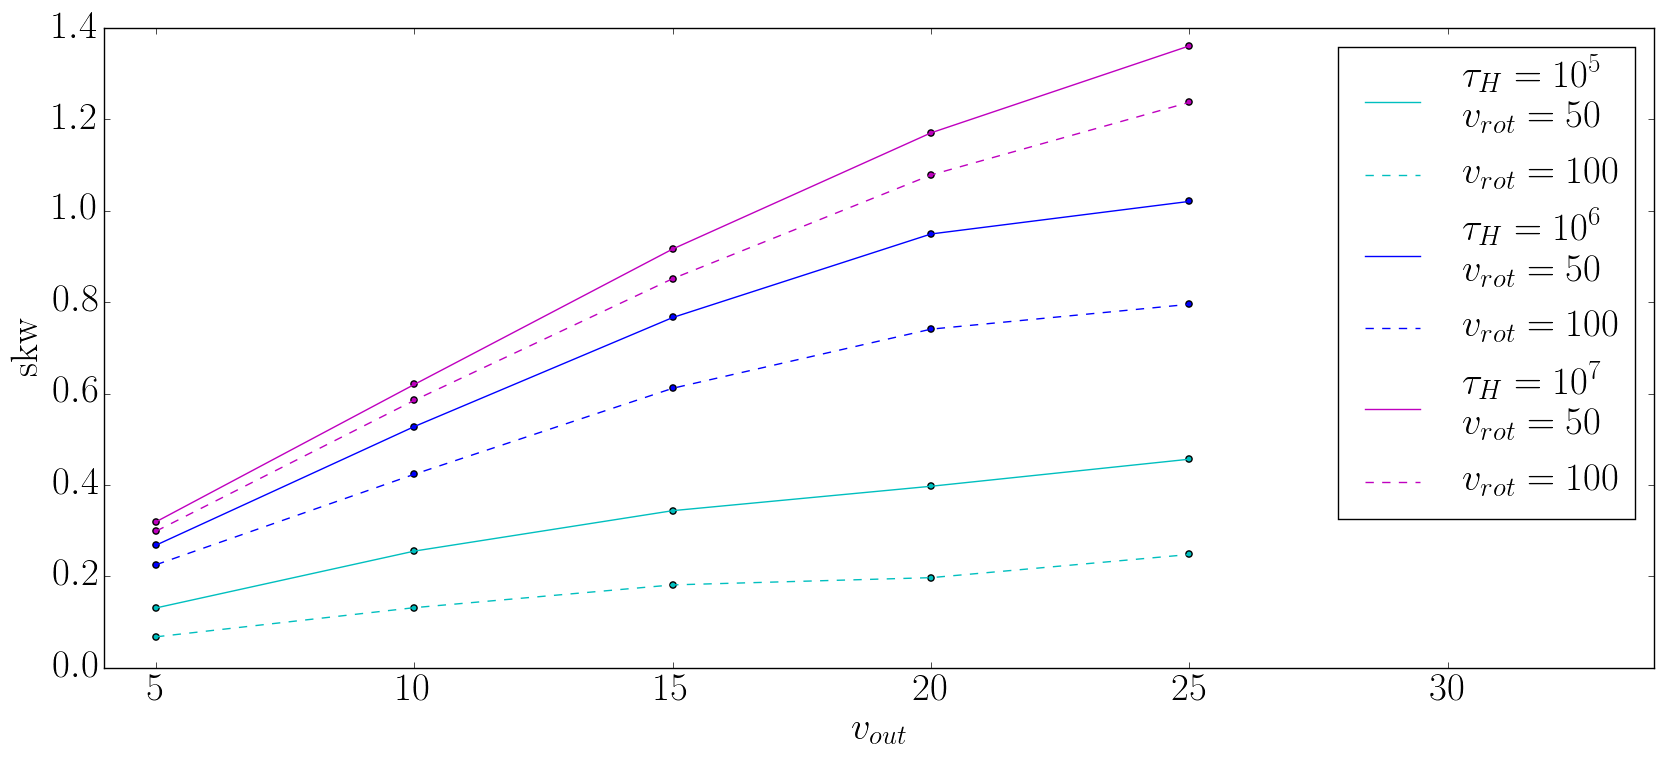
\includegraphics[width=1\textwidth]{./figures/chapter3/skw}
	\end{center}
	\caption{\textbf{Skewness plot for each \tauh.} The viewing angle $\theta \simeq 90^\circ$. 
		\label{fig:skw}}
\end{figure}

Fig. \ref{fig:skw} show that the skewness is proportional to the outflow velocity, at a fixed rotational velocity. The greater \vout is, the more asymmetric is the \lya frequency distribution. The horizontal dotted line is the value of skewness for Q2206BX151. As seen, the line intersects with the skewness curves. This would imply that Q2206BX151, according to the model, has its parameters narrowed to: \vrot $\in [50,100]$ \kms, \vout $\in [15,20]$ \kms and \tauh $\in [10^6, 10^7]$. However, these values are not completely consistent with the standard deviation.\\

\subsection{Sigma of Asymmetry}
Sigma of asymmetry $\sigma_A$ is another measure for the asymmetry of the \lya line. It was defined by McLinden et al. \cite{McLinden2011} as follows. The two peaks, the red one and the blue one, are fitted with a Gaussian curve. Their standard deviations $\sigma_{red}$ and $\sigma_{blue}$ are obtained. Then the factor $\sigma_A$ is:

\begin{equation}
\sigma_A = \frac{\sigma_{red}}{\sigma_{blue}}
\end{equation}

If the value is less than one, the left peak is thiner than the right peak. If it is greater than one, there left peak is wider than the right peak.\\

\begin{figure}[h!]
	\begin{center}
		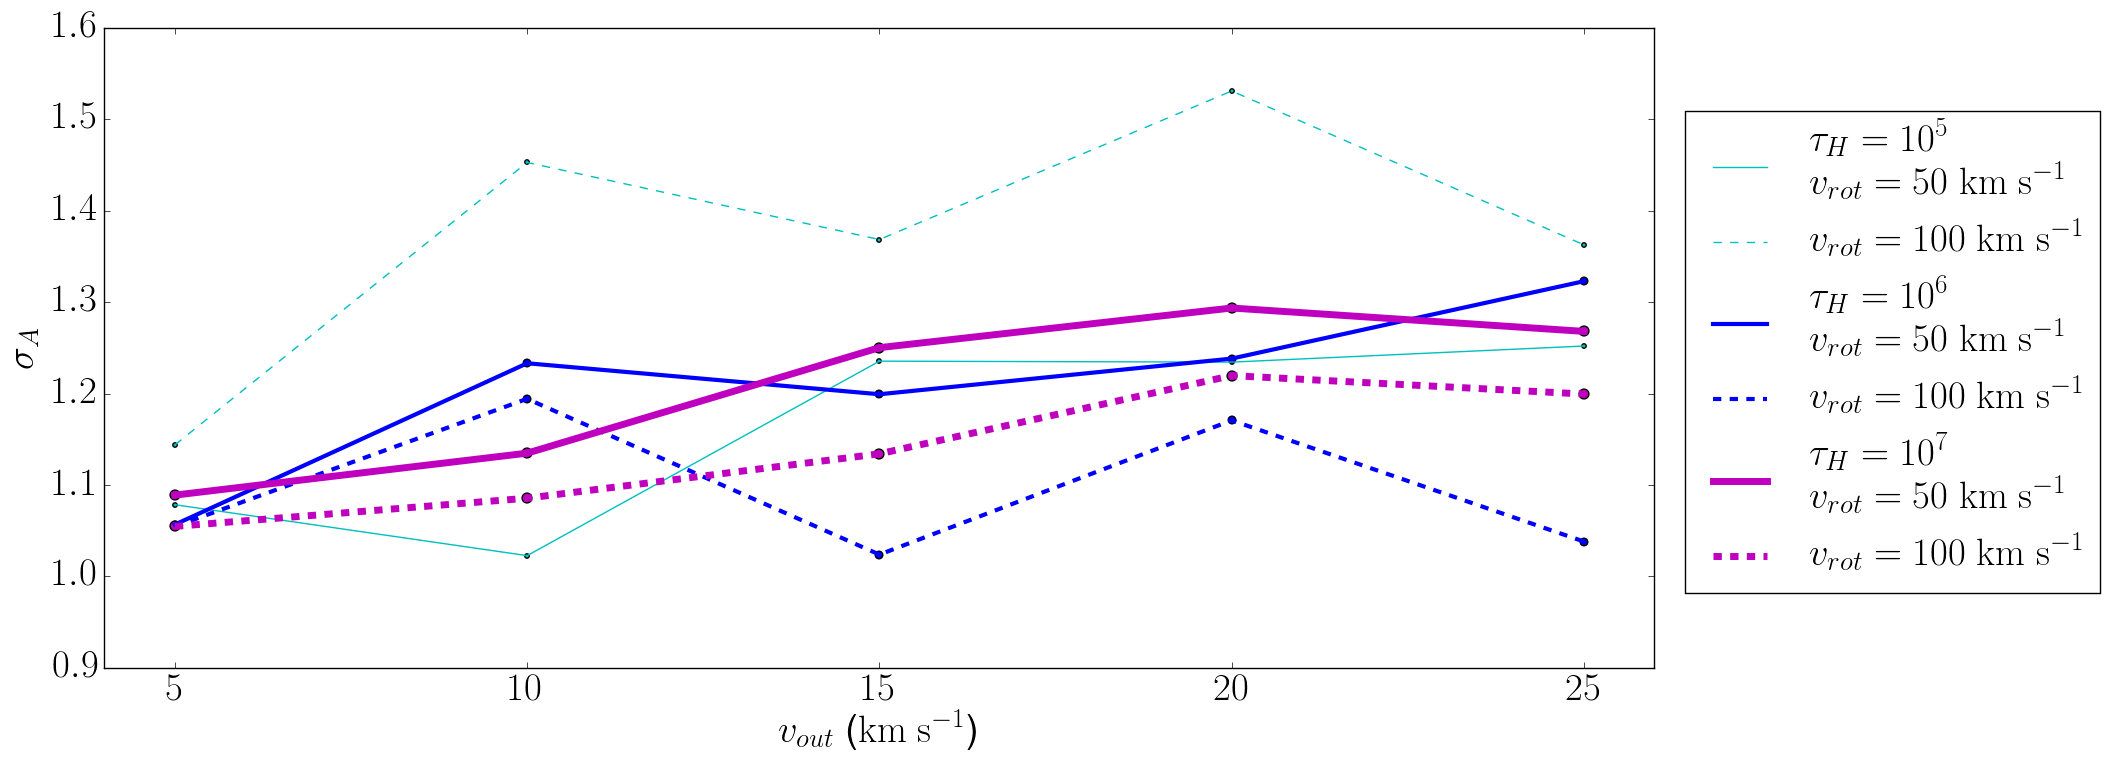
\includegraphics[width=1\textwidth]{./figures/chapter3/sigma}
	\end{center}
	\caption{\textbf{Sigma of asymmetry $\sigma_A$.} 
		\label{fig:sigma}}
\end{figure}

Fig. \ref{fig:sigma} shows that this parameters has high fluctuations. I can not see a clear behavior or tendency that applies to all the curves. The only thing is that the values of $\sigma_A$ start close together and \vout makes them separate.\\ 

\section{Influences of the free parameters}

To summarizem the influence of the 3 parameters on the \lya morphology is the following: 

\begin{itemize}
\item \tauh induces a redshift. Increasing the optical depth separates the line of the zero velocity line. \\
\item \vout decreases the right peak's intensity. Higher \vout make the left peak smaller until it merges with the right one. \\
\item \vrot broadens the line and decreases the maximum intensity. Higher \vrot implies a flatter spectrum. This effect has not been deeply studied in literature. Only Garavito et al. \cite{Garavito14} has simulated its effect. Our results are consistent with their conclusions. \\
\end{itemize}